% !TeX root = ../main.tex
\chapter{动态排队服务中的规划蒸馏与反事实辅助协同控制}
\label{cha:whole-system}
\label{cha:ch5-dynamic}

\section{研究问题与协议边界}
\label{sec:whole-method}
\label{sec:ch5-motivation}

\subsection{从批量分配到跨时隙排队}

第三章说明需求可见性如何影响无人机集群的覆盖接纳，第四章进一步刻画给定位置与请求集合时的批量资源竞争。对于连续到达的计算服务，当前位置和本次分配还会改变后续传输、CPU 排队与截止期损失。若只评价当前批次，可能偏好立即增加接纳，却没有为已接纳请求保留足够的传输与执行机会。本章因此研究突发请求驱动的动态排队服务，重点考察如何把已有规划知识转化为较快的联合控制策略，以及环境交互能否继续改善蒸馏得到的策略初值。

为隔离跨时隙传输与计算的影响，本章采用独立的动态排队服务协议。该协议保留五架 UAV、一百个 UE、一个 MBS、$100\,\mathrm{m}$ 物理服务半径及规定机动范围，但采用固定 UE 几何、可跨时隙保留的请求进度和节点 EDF 执行。它不是第三、四章含缓存、能量与最终批量算力均分模型的直接延长。特别是，本章未引入 UAV 推进能耗、通信能耗、UE 无线供能及电池动态，不能用本章 DSR 的绝对值与前两章作直接数值比较，也不能据此宣称含能耗约束的完整系统已被联合优化。

本章提出的具体方法由三个环节构成。首先，以有限候选规划器提供监督目标，通过两轮数据聚合获得联合策略的蒸馏初值。其次，在完整环境轨迹上训练价值网络，并把共同随机数下的短视界反事实评分作为 Actor 辅助更新信号，进行联合 PPO 微调。最后，根据在线计算预算，使用零在线 Engine 前瞻策略直接选择联合动作，或使用学习先验引导 Top-6 候选的三步 MPC。前者仍需候选生成与解析排队特征计算，后者还需环境克隆前瞻；两者都在后续实验中测量完整决策调用的墙钟耗时。

本章检验两个主要问题：完整微调方案能否改善蒸馏学生初值，学习引导 Top-6 MPC 能否相对指定在线规划基线改善服务质量与平均计算成本。跨层条件化和期望向量是所设计策略的组成部分，其独立性能贡献另用匹配消融考察，不预设所有组件均有显著收益。PPO、广义优势估计和数据聚合分别沿用已有方法思想\cite{schulman2017proximal,schulman2015high,ross2011dagger}，本章的贡献定位于该排队任务下的联合表示、训练组合与控制方式。

\subsection{与第三、四章的联系及区别}

表~\ref{tab:ch5-protocol-boundary} 将章节联系落实到模型和证据层面。三章共同关注请求如何进入服务以及能否按时完成，但分别回答需求观测、固定快照分配和持续排队控制问题。第四章的 MC-ITR 既没有作为本章在线下层，也没有用作本章蒸馏教师。历史共享快照桥接仍是第四章协议下的离线分配比较，不能与本章闭环增益相加。

\begin{table}[!htbp]
\centering\small
\bicaption{第三、四章与本章的协议和证据边界}{Protocol and evidence boundaries across Chapters 3--5}
\label{tab:ch5-protocol-boundary}
\begin{tabularx}{\textwidth}{lYY}
\toprule
项目 & 第三、四章 & 本章 \\
\midrule
研究对象 & 需求感知轨迹；固定快照批量分配 & 突发到达下的跨时隙联合控制 \\
执行模型 & 原通信、缓存与最终批量共享算力 & 上传、转发和 EDF 计算的持续队列 \\
UE 与请求 & 原用户移动、服务及能量请求机制 & 固定 UE 几何，带属性的时隙泊松计算请求 \\
能量因素 & 按原协议记录 UAV 能耗与 UE 能量状态 & 未建立推进、通信、WPT 或电池动态 \\
控制策略 & Attention-MAPPO；MC-ITR 快照求解 & 候选级联合策略、反事实辅助 PPO、Top-6 MPC \\
可比较范围 & 各自协议内的配对对照 & 相同排队协议和确认工作负载内的对照 \\
\bottomrule
\end{tabularx}
\end{table}

\section{动态服务系统与候选动作建模}
\label{sec:ch5-queue-model}

\subsection{突发到达、任务属性与完整结算}

每个评估回合包含 $200\,\mathrm{s}$ 的请求生成阶段，宏决策步长为 $1\,\mathrm{s}$。每个工作负载固定一组 UE 位置和空间需求热点演化，任务可以在同一 UE 同一时隙重复产生。时隙泊松批次的期望总到达率为
\begin{equation}
 \lambda(t)=\begin{cases}
 15,&0\leq t<50,\\
 60,&50\leq t<100,\\
 15,&100\leq t<200,\\
 0,&t\geq200.
 \end{cases}
 \label{eq:ch5-arrival}
\end{equation}
图~\ref{fig:ch5-dynamic-protocol} 展示该负载设计。它是合成业务协议，不是应急现场的实测流量记录。任务输入大小在 $1.5\times10^6$ 至 $3.0\times10^6$ bytes 之间取整数，计算密度在 $500$ 至 $1000$ cycles/bit 之间取整数。令输入比特数为 $b_n$、计算密度为 $\omega_n$，则计算量 $c_n=b_n\omega_n$。期限相对到达时刻在 $[2,3]\,\mathrm{s}$ 内生成。

\begin{figure}[!htbp]
\centering
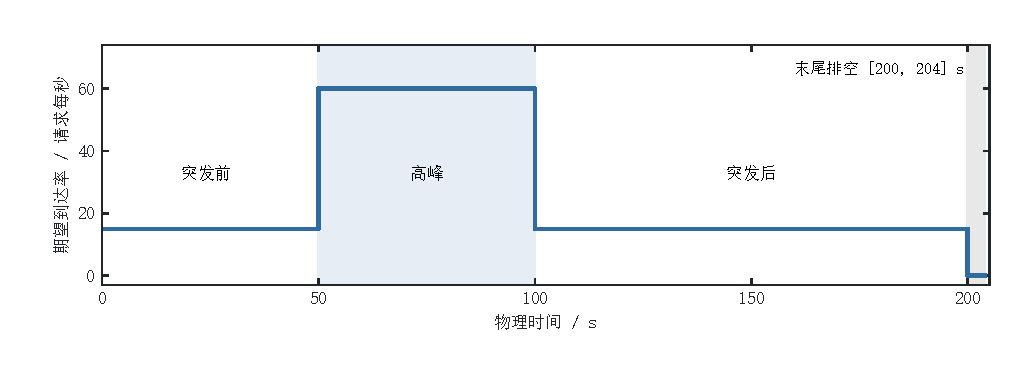
\includegraphics[width=0.94\textwidth]{../docs/figures/ch5_dynamic_01_protocol.pdf}
\bicaption{动态排队协议的期望到达率与排空阶段。阴影标出 $50$--$100\,\mathrm{s}$ 高峰窗口；$200\,\mathrm{s}$ 后停止生成请求，并继续结算未完成队列。曲线表示预设期望强度，不是观测流量拟合}{Prespecified arrival intensity and the post-arrival drain stage}
\label{fig:ch5-dynamic-protocol}
\end{figure}

停止到达后仍继续选择动作并推进系统，直到请求全部完成或过期。冻结实现对宏步起点采用 $t\leq204$ 的保护检查，实际终止由队列是否为空决定。该处理使最后阶段产生的请求也获得完整结算，避免只在 $t<200$ 统计成功而截断晚到请求。训练经验同样保留排空步自身的状态、动作、旧策略概率和奖励，而不是把排空阶段收益事后合并到最后一个活跃步。

设回合生成、接纳、按时完成的请求数分别为 $G,A,S$，主指标定义为
\begin{equation}
 \mathrm{DSR}=\frac{S}{G},\qquad
 P_{\mathrm{adm}}=\frac{A}{G},\qquad
 P_{\mathrm{done}\mid\mathrm{adm}}=\frac{S}{A},\qquad
 \mathrm{DSR}=P_{\mathrm{adm}}P_{\mathrm{done}\mid\mathrm{adm}}.
 \label{eq:ch5-dsr-identity}
\end{equation}
该恒等式只在使用同一组请求计数时成立。分阶段结果按请求到达时间归入突发前、高峰和突发后队列，完成时刻可以晚于所属窗口；非高峰汇总突发前和突发后两组。所有实际生成请求都进入分母，包括一直未被接纳而过期的请求。完整排空后 $G=S+E$，其中 $E$ 为过期请求数。

\subsection{不可变关联与传输--计算串联队列}

请求 $n$ 的运行状态包含到达时刻 $a_n$、绝对截止时刻 $d_n$、来源 UAV、执行节点，以及剩余上传量、转发量和计算周期。未覆盖请求处于等待状态，若在截止前进入服务范围，才由最近 UAV 首次接纳；首次来源确定后不再切换。控制器只对新接纳且尚未分配的请求选择执行目标，目标一旦确定也不再迁移。因而，当前动作不能任意重排历史任务的执行节点，只能影响新分配和后续服务几何。

每个任务依次经历等待覆盖、UE 上传、必要的 UAV 间转发或 MBS 回传、目标节点计算。上传或转发因失去连接而暂停时，已完成进度保留；通信完成后才释放到 CPU 队列。记节点 $j$ 的就绪任务集合为 $\mathcal C_j(\tau)$，其执行规则为
\begin{equation}
 n_j^*(\tau)=\mathop{\arg\min}_{n\in\mathcal C_j(\tau)}(d_n,\mathrm{uid}_n),\qquad
 f_n(\tau)=F_j\mathbf1\{n=n_j^*(\tau)\}.
 \label{eq:ch5-edf}
\end{equation}
这里 EDF 表示最早截止期优先，同期限按任务标识排序，允许新就绪的更早截止任务抢占。UAV 算力依次为 $(75,60,70,85,50)\times10^9$ cycles/s，MBS 为 $200\times10^9$ cycles/s。式~\eqref{eq:ch5-edf} 与第四章按最终批量均分算力的模型不同，不能混用其负载预测或局部最优性质。

通信速率按几何关系和香农型链路模型计算。每个 UE 同时上传其最紧迫任务，同一来源 UAV 下活跃 UE 共享上传带宽；协作链路与回传链路分别在活跃有向节点对之间共享资源。覆盖半径为 $100\,\mathrm{m}$，感知与 UAV 协作距离均为 $460\,\mathrm{m}$。上传、协作与回传带宽分别为 $40$、$20$ 和 $0.75\,\mathrm{MHz}$。发送功率是链路速率模型的参数，不代表本章已经积分结算通信能耗。

UAV 保持 $100\,\mathrm{m}$ 高度，水平位置位于 $[50,650]^2\,\mathrm{m}^2$，每步位移模长至多 $15\,\mathrm{m}$。执行器沿线性运动路径检查 $200\,\mathrm{m}$ 最小机间距，并在覆盖或协作接触边界、任务完成和截止事件处结算。该检查针对本章的理想线性位移模型，不包含飞行动力学、姿态和控制误差。

\subsection{可用信息、候选库与状态特征}

控制器观察当前 UAV 位置、已接纳任务的剩余服务状态，以及机群感知范围内 UE 的待接纳请求。它使用历史可见到达计数估计需求强度，不读取随后真实发生的请求批次。执行时采用集中候选级决策：候选卸载方案给出本步新请求的目标节点，候选运动给出五架 UAV 的联合位移。这里的上下层指分配与运动两个决策分支，不是直接复用第三章的分散 Attention-MAPPO。

记候选分配集合为 $\mathcal K(s)$、候选运动集合为 $\mathcal M(s)$，联合动作是 $(k,m)$。候选构造调用冻结的上游提案器和评分器，并加入安全分配与待接纳需求救援方向。合法运动需满足全路径几何约束。本章研究有限候选集上的选择，未声称覆盖所有连续轨迹及离散分配。初始先验选择器虽然没有训练本章新增的选择网络，仍依赖这些上游学习模型与启发式，不能视为完全不含先验知识的随机系统。

分配特征 $\mathbf a_k\in\mathbb R^{14}$ 包含节点计算负载、可完成量、溢出风险、转发比例及先验信息；运动特征 $\mathbf m_{km}\in\mathbb R^{16}$ 结合覆盖救援、预测到达服务能力、排队风险、位移和方案依赖信息；上下文 $\mathbf c\in\mathbb R^{14}$ 汇总历史到达估计和当前队列压力。特征通过解析评价获得，无需为每个候选克隆执行 Engine，但并非没有在线计算成本。

\section{规划知识蒸馏与候选级联合策略}
\label{sec:ch5-distillation}

\subsection{考虑释放时间的排队近似}

传输尚未完成的请求不能提前占用 CPU。若把按截止期排序的所有请求直接串行预约到节点时间线上，可能让未就绪任务挡住已经可计算的任务。为避免这一类跨阶段预约偏差，特征计算先估计上传与转发完成时刻，作为 CPU 释放时间 $r_{nj}$，再在每个节点上对已经释放的任务进行工作守恒 EDF 推进。当前任务完成、更早截止任务到达 CPU 或任务过期，都会触发下一次事件选择。

该过程输出近似可完成量 $\widehat C(s,k,m)$ 和溢出量 $\widehat O(s,k,m)$，用于候选特征及后续状态势评价。输出可以包含实现中对三步窗口以外完成的折减，因而是评分特征，不是整数成功数的替代计数器。实际成功数始终由完整 Engine 执行记录确定。该近似还依赖代表性几何、带宽共享和等待请求接纳估计，不具有一般精确排队求解保证。

在 $932$ 个验证动作对上，释放时间近似与三步 Engine 参照的相关系数为 $0.9996$，平均绝对误差为 $0.2758$；旧单次 Lindley 近似对应 $0.99963$ 和 $0.2704$。新近似修正了构造反例中的就绪顺序问题，但该验证集的整体误差没有降低。因此，较高相关性只支持其在所检验状态上的数值接近性，不证明普遍优于旧近似，更不证明候选最优动作始终一致。

\subsection{双分支联合分布与期望反馈}

运动分支先对每个方案的候选运动评分。令 $p^0_m(m\mid s,k)$ 为正值先验，$g_m$ 为带线性跳连的单隐层评分网络，则
\begin{equation}
 p_{\theta_m}(m\mid s,k)=\operatorname{softmax}_{m}
 \left[\log p_m^0(m\mid s,k)+g_m([\mathbf m_{km},\mathbf a_k,\mathbf c])\right].
 \label{eq:ch5-motion-policy}
\end{equation}
评分网络为 $g(\mathbf x)=\mathbf x^\top\mathbf w+\tanh(\mathbf x^\top W+\mathbf b)^\top\mathbf v$，隐层宽度为48。取运动特征前四维构成 $\boldsymbol\phi_{km}$，分别表示规范化救援潜力、预测到达服务量、排队溢出风险和净服务评分，定义
\begin{equation}
 \mathbf C_{\mathrm{upper}}(s,k)=\sum_{m\in\mathcal M(s)}
 p_{\theta_m}(m\mid s,k)\boldsymbol\phi_{km}.
 \label{eq:ch5-coupling}
\end{equation}
分配分支再使用该期望向量，构造
\begin{equation}
 \begin{aligned}
 p_{\theta_a}(k\mid s)&=\operatorname{softmax}_{k}
 \left[\log p_a^0(k\mid s)+g_a([\mathbf a_k,\mathbf C_{\mathrm{upper}}(s,k),\mathbf c])\right],\\
 \pi_\theta(k,m\mid s)&=p_{\theta_a}(k\mid s)p_{\theta_m}(m\mid s,k).
 \end{aligned}
 \label{eq:ch5-joint-policy}
\end{equation}
两个分支输入维度分别为32和44。分配概率对 $\mathbf C_{\mathrm{upper}}$ 的依赖，使分配损失可以沿式~\eqref{eq:ch5-coupling} 回传到运动分支。它是一个明确的参数耦合设计，而不是关于该结构性能必然占优的理论保证。

严格去耦对照把全部八个方案相关运动通道以及方案特征按下层先验边缘化，运动先验也替换为 $\bar p_m^0(m\mid s)=\sum_kp_a^0(k\mid s)p_m^0(m\mid s,k)$，并令 $\mathbf C_{\mathrm{upper}}=0$，从而得到 $\pi(k,m\mid s)=p_a(k\mid s)p_m(m\mid s)$。保存模型在验证状态上的跨方案运动概率差实测为零。仅去掉期望向量的对照则保留 $p_m(m\mid s,k)$ 的方案条件化，不能与严格去耦混称。

\subsection{规划教师目标与两轮数据聚合}

策略蒸馏将较昂贵策略的输出作为学生监督目标\cite{rusu2015distillation}。本章教师对候选联合动作执行既有三步规划评分，并结合预测到达服务能力、原排队近似、过载与救援规则形成 $Q_T(s,k,m)$。教师评分仍包含启发式修正；本节的释放时间近似主要用于新学生特征和状态势，不能据此宣称教师已被替换为精确排队求解器。

教师分布以方案和运动先验乘积为基准，按得分指数重加权：
\begin{equation}
 \begin{aligned}
 u_T(s,k,m)&=\operatorname{clip}\left[
 \frac{Q_T(s,k,m)-Q_T^{\max}(s)}{\tau},-60,0\right],\\
 q_T(k,m\mid s)&=\frac{p_T^0(k,m\mid s)\exp u_T(s,k,m)}
 {\sum_{k',m'}p_T^0(k',m'\mid s)\exp u_T(s,k',m')},
 \qquad\tau=0.015.
 \end{aligned}
 \label{eq:ch5-teacher}
\end{equation}
学生最小化教师到学生的 KL 散度。联合蒸馏与去耦蒸馏使用相同联合目标，区别在学生表达结构，而非给联合学生更好的教师标签。

借鉴数据聚合思想\cite{ross2011dagger}，第一轮在初始先验和均匀候选探索形成的轨迹上采集状态；第二轮由第一轮联合学生运行，补充其诱导状态上的教师标注，再聚合两轮训练集继续拟合。每轮最多32个训练 epoch、批大小16、初始学习率0.008，按验证集教师 KL 选择蒸馏检查点。该两轮方案用于减小监督状态分布与学生闭环状态之间的偏差，不直接继承一般 DAgger 理论所需条件下的全部性能保证。

蒸馏阶段允许调用教师规划器，测试时学生不调用教师。此处的收益首先是计算摊销：把训练时取得的候选偏好编码到学生分布。监督目标不能保证学生在长期闭环中最优，因此后续使用完整环境交互继续优化，而不把教师或学生初值当作性能上界。

\section{环境交互与反事实辅助 PPO 微调}
\label{sec:ch5-rl}

\subsection{完整真实轨迹奖励与状态价值}

真实环境轨迹按照所采样的联合动作执行分配及运动。令 $\Delta S_t$、$\Delta E_t$ 和 $\Delta D_t$ 分别为一步新增成功、过期和断链事件数，冻结实现采用
\begin{equation}
 r_t=\Delta S_t-0.65\Delta E_t-0.05\Delta D_t
 +\Phi_{\mathrm{post}}(s_t^+)-\Phi_{\mathrm{pre}}(s_t).
 \label{eq:ch5-real-reward}
\end{equation}
$s_t$ 是动作前已加入本步到达并完成接纳的状态，$s_t^+$ 是本步执行后的状态，尚未加入下一步新到达。$\Phi_{\mathrm{pre}}$ 只评价已接纳任务；$\Phi_{\mathrm{post}}$ 还把新位置覆盖内的待接纳任务作虚拟本地接纳估计。两者均基于释放时间近似，其形式为
\begin{equation}
 \Phi=0.65\widehat C-0.65\widehat O
 -0.35\sum_{u=1}^{5}[\ell_u-1]_+^2,\qquad
 \ell_u=\sum_{n\,\mathrm{assigned\ to}\,u}\frac{c_n^{\mathrm{rem}}}{F_u}.
 \label{eq:ch5-potential}
\end{equation}
动作前未分配的已接纳任务按来源本地处理，动作后的虚拟接纳也按本地处理；队列为空时该评分取零。式~\eqref{eq:ch5-real-reward} 的势差没有乘折扣因子，且前后评价对象不同。因此本章把它作为任务相关奖励塑形，不主张具有标准折扣势塑形的策略不变性。训练优化的折扣塑形回报与最终 DSR 也不完全相同，二者关系需由独立评估确认。

价值网络 $V_\psi$ 的输入为34维，分别由14维上下文、分配特征的6维先验均值和4维最大值、运动特征的6维先验均值和前4维最大值组成；隐层宽度48。对包括排空步的完整轨迹，使用 $\gamma=0.85$、$\lambda_{\mathrm{GAE}}=0.90$ 计算\cite{schulman2015high}
\begin{equation}
 \delta_t=r_t+\gamma V_\psi(s_{t+1})-V_\psi(s_t),\qquad
 \widehat A_t=\delta_t+\gamma\lambda_{\mathrm{GAE}}\widehat A_{t+1},\qquad
 \widehat R_t=\widehat A_t+V_\psi(s_t).
 \label{eq:ch5-gae}
\end{equation}
真实终止处下一状态值和后续优势取零。Critic 用真实轨迹的 $\widehat R_t$ 训练，采用阈值5的 Huber 损失与参数正则；反事实评分不作为 Critic 标签。这一分离限制了辅助评分对价值拟合的直接影响，但不构成 GAE 估计无偏性的保证。

\subsection{共同工作负载基线与短视界反事实评分}

同一工作负载和时间下的两个动作流提供留一法辅助基线。对动作流 $i$，先计算
\begin{equation}
 \widetilde A_{i,t}=\widehat A_{i,t}
 -\frac{0.5}{N_t-1}\sum_{j\neq i}\widehat A_{j,t},\quad N_t\geq2,
 \label{eq:ch5-loo}
\end{equation}
再在更新数据中作均值--标准差规范化，并裁剪到 $[-4,4]$。只存在一个流时不使用留一基线。Critic 更新后重新计算轨迹优势，再用于 Actor 更新。相同外生工作负载减少到达差异，但动作引起的状态分歧仍然保留。

微调期间每隔四个活跃步，从旧策略分布构建至多四个反事实联合动作。候选集合为已执行动作与确定性 Top-3 动作的并集；若不足四个，再抽取一个均匀随机索引加入集合，重复索引可能使集合仍不足四个。因此，它不是四个独立同分布的旧策略样本。

每个候选从同一个公开状态克隆 Engine，先执行该候选的一步分配和运动，再使用安全分配与零位移继续两步。两步未来到达由历史可见需求的三步滑窗估计生成，候选共享完全相同的预测批次，即共同随机数（CRN）。这里的未来是预测样本，不是实际工作负载的未来真值，后续控制也不是待训练联合策略的完整延续。

必须区分反事实评分与式~\eqref{eq:ch5-real-reward}。记克隆分支新增成功、过期、断链为 $\Delta S^{(3)},\Delta E^{(3)},\Delta D^{(3)}$，$U^{(3)}=\max(A^{(3)}-S^{(3)},0)$ 为克隆累计已接纳但未成功的计数，其中可能包括已过期任务；$R_{\mathrm{rescue}}(s,m)$ 为运动救援价值。辅助评分是
\begin{equation}
 Q_{\mathrm{cf}}(s,k,m)=\Delta S^{(3)}-0.65\Delta E^{(3)}-0.05\Delta D^{(3)}
 -\eta(s)U^{(3)}+\zeta(s)R_{\mathrm{rescue}}(s,m),
 \label{eq:ch5-cf-score}
\end{equation}
拥塞时 $(\eta,\zeta)=(0.45,0)$，否则为 $(0.15,0.25)$。该评分不包含真实轨迹的前后势差，不能写成式~\eqref{eq:ch5-real-reward} 的三步累加回报。它是结合物理执行器与启发式末端项的模型辅助评分。

对当前候选组 $\mathcal B_t$，构建
\begin{equation}
 \widehat A_{\mathrm{cf}}(s,b)=\operatorname{clip}\left(
 \frac{Q_{\mathrm{cf}}(s,b)-\overline Q_{\mathcal B_t}}
 {\max(\operatorname{std}_{b'\in\mathcal B_t}Q_{\mathrm{cf}}(s,b'),0.10)},-3,3\right).
 \label{eq:ch5-cf-adv}
\end{equation}
评分无差异时不加入辅助样本。组中心化用于强调相同状态下的相对候选质量，不能将其解释为真实长期价值函数的无偏优势估计。

\subsection{联合裁剪目标与训练组合}

Actor 沿用 PPO 裁剪形式\cite{schulman2017proximal}。对联合动作 $b=(k,m)$，定义
\begin{equation}
 \begin{aligned}
 \rho_\theta(s,b)&=\frac{\pi_\theta(b\mid s)}{\pi_{\mathrm{old}}(b\mid s)},\qquad\epsilon=0.20,\\
 \ell_{\mathrm{clip}}(s,b,A)&=-\min\{\rho_\theta A,
 \operatorname{clip}(\rho_\theta,1-\epsilon,1+\epsilon)A\}.
 \end{aligned}
 \label{eq:ch5-ppo}
\end{equation}
真实轨迹条目使用规范化后的 $\widetilde A$，反事实条目使用 $1.25\widehat A_{\mathrm{cf}}$。实现将两类条目合并后按批平均，同一状态可因多个辅助候选而重复出现。每个条目的损失还包含 $-\beta_H H(\pi_\theta)$、$\beta_{\mathrm{KL}}D_{\mathrm{KL}}(\pi_{\mathrm{ref}}\|\pi_\theta)$ 与参数正则。微调以蒸馏初值作为参考锚点，冷启动以候选先验为锚点。

真实轨迹中的动作由旧策略采样，但反事实集合还包含确定性 Top-3，代码未为这种候选选取分布另作抽样修正。因此，本章将总体算法称为\emph{环境交互与反事实辅助 PPO}，其中辅助项是一种偏置的模型辅助优化目标，不把整个混合更新称为标准在策略 GRPO，也不赋予其标准 PPO 的无偏策略梯度解释。其有效性以完整方案的闭环比较为依据。

\begin{table}[!htbp]
\centering\small
\bicaption{冷启动与蒸馏暖启动微调的冻结训练参数}{Frozen configurations for scratch training and distilled warm-start fine-tuning}
\label{tab:ch5-dynamic-hyper}
\begin{tabular}{lrr}
\toprule
配置项 & 冷启动 & 暖启动微调 \\
\midrule
Actor 学习率 & 0.0035 & 0.0025 \\
Critic 学习率 & 0.008 & 0.008 \\
Actor / Critic epoch & 6 / 10 & 4 / 8 \\
批大小 & 32 & 64 \\
熵系数 $\beta_H$ & 0.002 & 0.0005 \\
KL 系数 $\beta_{\mathrm{KL}}$ & 0.015 & 0.015 \\
反事实间隔 / 优势权重 & 关闭 / 0 & 4步 / 1.25 \\
折扣 $\gamma$ / GAE $\lambda$ & 0.85 / 0.90 & 0.85 / 0.90 \\
更新轮次 / 每轮真实回合数 & 4 / 12 & 4 / 12 \\
\bottomrule
\end{tabular}
\end{table}

每个训练臂、每个父谱系执行四轮更新，每轮使用六个工作负载的两个动作流，共12条真实轨迹，累计48回合。反事实分支会增加额外训练计算，并不包含在48条真实轨迹的计数中。表~\ref{tab:ch5-dynamic-hyper} 表明冷暖组同时改变初始化、辅助项、参考锚点和优化参数，比较所识别的是完整训练组合，而不是暖启动单因子的纯效应。耦合微调与无期望向量微调从相同联合蒸馏检查点开始，但策略结构开关仍可能使初始动作分布不同。

\begin{algorithm}[!htbp]
\small
\caption{规划蒸馏与环境交互、反事实辅助 PPO 微调}
\label{alg:ch5-dynamic-training}
\KwIn{冻结候选提案器、评分器，训练与验证工作负载，联合策略结构}
\KwOut{验证集选择的联合微调策略}
在先验与探索轨迹采集状态，计算教师候选分布，训练第一轮学生\;
由第一轮学生运行并补充教师标注，聚合两轮数据继续蒸馏\;
复制蒸馏 Actor，初始化 Critic，固定蒸馏参考策略\;
\For{四轮 PPO 更新}{
  在六个训练工作负载及两个动作流上收集完整真实轨迹\;
  保留活跃阶段和全部非空队列排空步的状态、动作、概率与奖励\;
  每四个活跃步构建至多四个候选，以共享预测到达执行三步反事实评分\;
  用真实轨迹 GAE 目标训练 Critic，重新计算规范化轨迹优势\;
  合并真实条目和组相对辅助条目，更新联合 Actor\;
  在独立验证工作负载上评估当前策略\;
}
按各谱系验证 DSR 从严格正更新轮次中选择检查点，冻结后执行确认评估\;
\end{algorithm}

\section{零在线前瞻与神经引导 Top-6 MPC}
\label{sec:ch5-deployment}

\subsection{零在线 Engine 前瞻策略}

第一种控制方式在当前观察上构建候选库与解析特征，按式~\eqref{eq:ch5-joint-policy} 采样联合动作，并仅在实际环境中执行该动作。测试采样温度为1.0，不为候选调用 Engine 克隆前瞻，也不重新查询离线教师。它把更多规划计算移到蒸馏和微调阶段，但仍执行上游网络、候选构造、安全启发式与释放时间排队近似，因此不能描述为只有一次纯神经网络前向计算。

第二种控制方式允许一定在线前瞻，把学习分布用于缩小候选搜索范围，并参与最终评分。两种方式共享任务语义和动作接口，提供不同的测试期开销选择；本章不设定未经测量的机载处理器算力，也不据仿真推断直接承诺硬实时控制。

\subsection{熵校准先验与三步候选评价}

令提议分布为 $p(k,m)$，首先计算其熵与幂次
\begin{equation}
 \begin{aligned}
 H(p)&=-\sum_{k,m}p(k,m)\log p(k,m),\\
 \alpha&=\min\{1,\max[0.25,H(p)/1.85]\},\\
 \widetilde p(k,m)&=\frac{p(k,m)^\alpha}{\sum_{k',m'}p(k',m')^\alpha}.
 \end{aligned}
 \label{eq:ch5-entropy-calibration}
\end{equation}
校准使用数值下界 $10^{-12}$。由于正幂保持概率顺序，它不改变非并列候选的 Top-6 排名，主要调整后续评分和并列选择所使用的先验强度。不能把熵校准本身解释为引入新的候选搜索能力。

选取 $\widetilde p$ 最大的至多六个联合动作，分别从相同公开状态克隆 Engine，并共享由历史预测生成的两批未来到达。首步执行候选，随后两步采用安全分配和悬停。记分支成功数为 $S^{(3)}$，则最终评价为
\begin{equation}
 J(s,k,m)=S^{(3)}-\eta(s)U^{(3)}+\zeta(s)R_{\mathrm{rescue}}(s,m)
 +0.65\log\widetilde p(k,m).
 \label{eq:ch5-mpc-score}
\end{equation}
评分按百分位精度四舍五入，最大分并列时按校准先验加权抽样。执行选中动作后，下一宏步用新观察重新构建候选并规划，而不是执行全部三步分支动作。

式~\eqref{eq:ch5-mpc-score} 与训练辅助式~\eqref{eq:ch5-cf-score} 也不相同，前者没有额外显式过期、断链扣分，却包含校准先验项。先验不仅影响哪些动作进入 Top-6，还影响保留动作的最终排序。因此，同框架对照用于检验\emph{学习先验参与筛选与评分的整体贡献}，不把差值单独解释为候选裁剪的因果效应。

\begin{algorithm}[!htbp]
\small
\caption{两种在线联合控制方式}
\label{alg:ch5-dynamic-control}
\KwIn{当前公开状态，冻结学生或微调策略，控制方式}
\KwOut{本步新请求分配及五机联合位移}
构建合法分配与运动候选，计算解析特征和联合提议分布\;
\eIf{使用零在线 Engine 前瞻方式}{
  按温度1.0的联合分布采样一个动作\;
}{
  根据分布熵校准先验，保留至多六个联合候选\;
  使用历史需求生成两批共享预测到达\;
  对每个候选执行首步动作及两步安全分配、悬停的克隆评价\;
  根据式~\eqref{eq:ch5-mpc-score} 选取最终动作\;
}
仅向实际服务环境提交本步动作，接收下一步观察\;
\end{algorithm}

\subsection{同框架对照和计算口径}

Top-6 MPC 设置三种提议来源：初始候选先验、联合蒸馏学生、联合微调策略。三者共用候选生成程序、预测随机数构造、三步评价和熵校准形式，分别记为先验、蒸馏和微调 Top-6 MPC。在线规划基线则使用原三步确定性规划与预测修正，候选救援门控和先验构造也与新 Top-6 路径存在差异。因此，后者是指定控制方案的整体参照，不是只改变搜索数量的一因子对照。

日志把在线规划基线的确定性 Engine 推进步数与 Top-6 的预测候选分支数分别记录。预测分支内部同样使用 Engine 克隆，不能因为其确定性计数栏为零就称为零仿真。只有候选选择方式中的零在线前瞻臂同时满足两类计数均为零。实际效率比较还需同时考虑候选生成、解析评分、网络和克隆评价的墙钟耗时。

\section{实验设置与确认结果}
\label{sec:ch5-experiments}

\subsection{数据划分、比较层级与统计单位}

本章主证据采用冻结版本 \texttt{queued\_joint\_rl\_v2\_20261106}。蒸馏和 PPO 使用940000--940011的十二个训练工作负载，前后六个分组分别用于两轮蒸馏，PPO 轮次交替使用两个六负载组；验证集为941000--941002。开发评估使用951000--951003，冻结后的确认集为955000--955007，三者不相互替代。模型检查点按验证结果选择，确认结果不用于选择迭代。

全部十七个评估臂在三个固定父谱系、八个确认工作负载和两个动作流上运行，共816个配对评估回合。每臂48回合，池化生成请求数均为252024。父谱系表示固定的上游模型及其后续选择器，不把这些评估回合或请求当成816次或25万次独立训练重复。冷启动、蒸馏、微调及同框架 MPC 的角色见表~\ref{tab:ch5-dynamic-main}。

全程 DSR 比较采用10000次配对分块 Bootstrap，重采样工作负载和动作流，并对三个固定父谱系的计数比率差求平均。该区间反映固定模型集合面对所评估外生负载的变化，没有重采样训练谱系，也没有估计重新训练上游模型的全部不确定性。确认前固定八项主比较，另披露全31项全程 DSR 比较的 Bonferroni 区间。接纳率、条件完成率和阶段指标作为解释性分析，其检验族不能自动等同于全程 DSR 的31项主口径。

冻结清单记录15个科学源码、6个上游父检查点和51个本实验模型的摘要；确认回合携带相应清单标识及开始时间。清单标识不等同于每个回合文件均有确认前内容摘要，已有回放审计也不等同于本次重新逐步复现训练。配套图表从816份原始回合计数与确认统计生成，原始训练和实验结果未因写作而改动。图源与来源索引保存在 \path{docs/figures/data/queued_joint_rl_20261106/}。

\subsection{验证曲线与全部评估臂}

图~\ref{fig:ch5-dynamic-validation} 显示当前预算下不同训练方案的验证变化。联合微调的平均验证 DSR 从47.63\%增至48.37\%，冷启动联合选择器则在约44\%附近波动。曲线支持两套训练流程呈现不同效果，但它包含不同初值、辅助信号和优化参数，不能据此将冷启动表现归因于唯一的长时域信用分配瓶颈。仅四轮更新的验证走势也不构成一般收敛性证明。

\begin{figure}[!htbp]
\centering
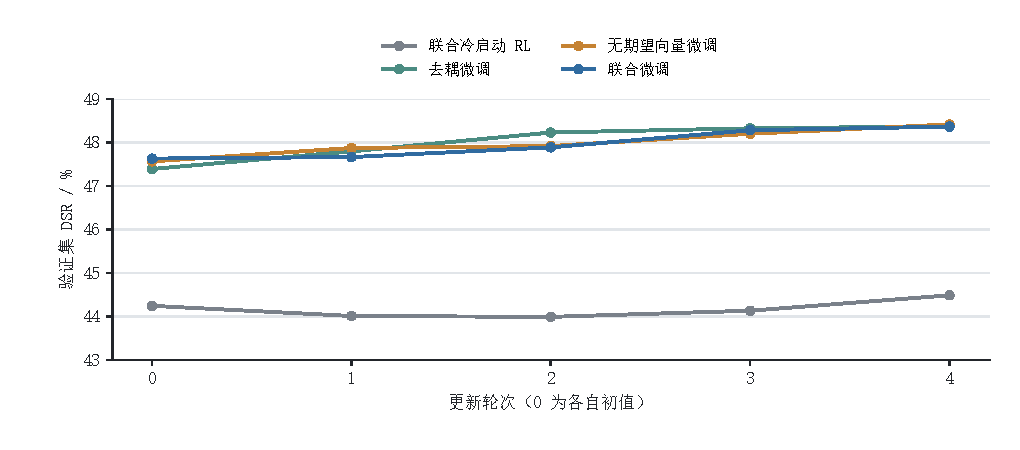
\includegraphics[width=0.96\textwidth]{../docs/figures/ch5_dynamic_02_validation.pdf}
\bicaption{训练方案的验证 DSR 曲线。各点来自三个父谱系的验证汇总，轮次0为各方案自身初值；验证工作负载与确认集独立。曲线比较整体流程，不是匹配初始化与辅助计算预算后的单因素试验}{Validation DSR across PPO updates for the evaluated training configurations}
\label{fig:ch5-dynamic-validation}
\end{figure}

\begin{table}[!htbp]
\centering
\bicaption{动态排队盲测确认集上全部十七种控制方案的服务性能对比}{Service performance of all seventeen control schemes on the dynamic-queue confirmation set}
\label{tab:ch5-dynamic-main}
\begin{tabular}{lrrrr}
\toprule
控制方案 & 按时完成数 $S$ & DSR/\% & 接纳率 $\alpha$/\% & 条件完成率 $\eta$/\% \\
\midrule
初始先验选择器 & $111,646$ & $44.30$ & $51.22$ & $86.48$ \\
仅下层 RL & $110,397$ & $43.80$ & $50.81$ & $86.21$ \\
仅上层 RL & $111,825$ & $44.37$ & $52.18$ & $85.04$ \\
单层训练后拼接 & $112,040$ & $44.46$ & $51.82$ & $85.78$ \\
去耦冷启动 RL & $111,328$ & $44.17$ & $52.02$ & $84.92$ \\
无期望向量冷启动 RL & $111,916$ & $44.41$ & $52.72$ & $84.23$ \\
联合冷启动 RL & $111,514$ & $44.25$ & $52.14$ & $84.87$ \\
去耦蒸馏 & $120,865$ & $47.96$ & $52.84$ & $90.76$ \\
无期望向量蒸馏 & $120,473$ & $47.80$ & $52.54$ & $90.98$ \\
联合蒸馏 & $121,079$ & $48.04$ & $52.42$ & $91.65$ \\
去耦微调 & $122,002$ & $48.41$ & $52.74$ & $91.79$ \\
无期望向量微调 & $122,571$ & $48.63$ & $52.81$ & $92.10$ \\
联合微调 & $122,842$ & $48.74$ & $52.58$ & $92.69$ \\
在线规划基线 & $122,382$ & $48.56$ & $51.76$ & $93.83$ \\
先验 Top-6 MPC & $114,573$ & $45.46$ & $48.90$ & $92.97$ \\
蒸馏 Top-6 MPC & $123,753$ & $49.10$ & $51.60$ & $95.17$ \\
微调 Top-6 MPC & $124,280$ & $49.31$ & $51.38$ & $95.98$ \\
\bottomrule
\end{tabular}
\sysutabnote{每种控制方案均在三组固定上游预训练模型、八个盲测工作负载和两个动作流（共 $48$ 回合、全集累计生成 $G=252{,}024$ 个请求）上配对评估。表内数值为全集累计请求计数比率（满足精确计数恒等式 $\mathrm{DSR}=\alpha\eta=(A/G)\times(S/A)$，例如联合微调 $122{,}842/252{,}024 = (132{,}524/252{,}024)\times(122{,}842/132{,}524) = 48.7422\%$，两位小数显示下 $52.58\%\times 92.69\%=48.736\%$ 的千分位尾差仅来自四舍五入显示）；单条请求与回合不作为独立训练重复样本。}
\end{table}


确认集的全部结果见表~\ref{tab:ch5-dynamic-main} 和图~\ref{fig:ch5-dynamic-arms}。初始先验选择器 DSR 为44.30\%，联合冷启动为44.25\%，联合蒸馏为48.04\%，联合微调为48.74\%。同一候选控制接口下，蒸馏和完整微调方案取得更高服务成功率。由于初始先验也使用上游学习模型和安全启发式，这里的冷启动仅指本章新增选择器的训练起点，不是从原始观测到动作的全系统零知识学习。

\begin{figure}[!htbp]
\centering
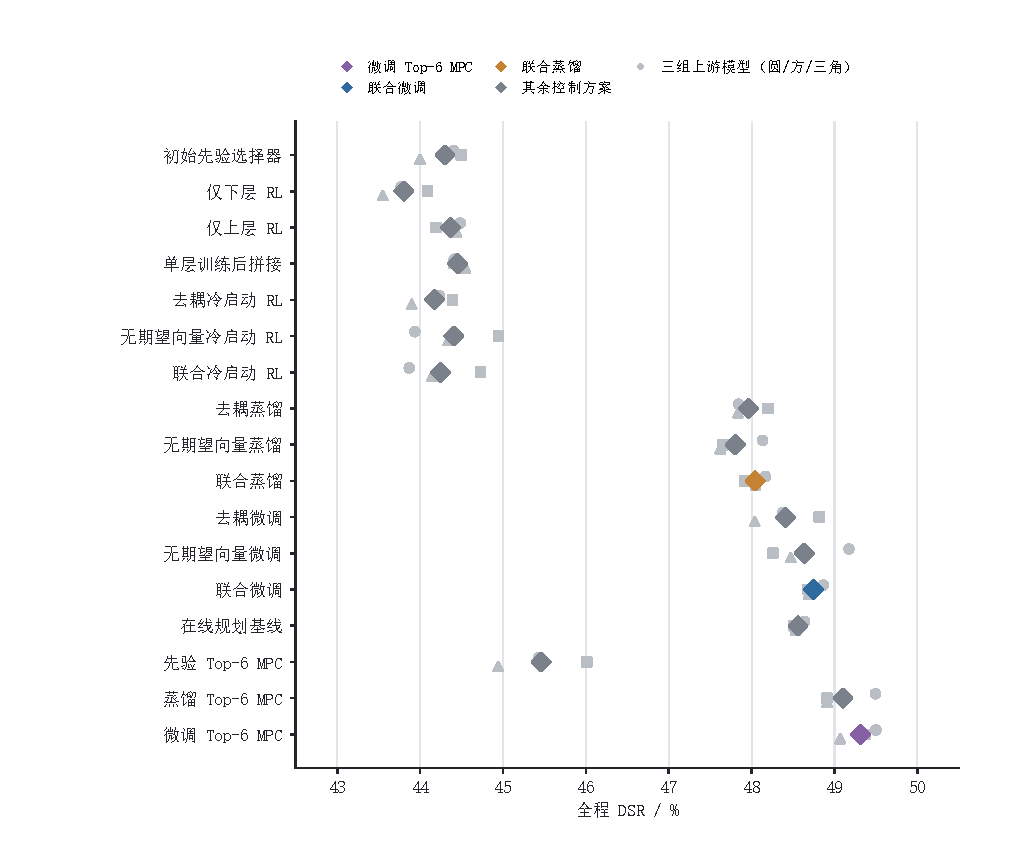
\includegraphics[width=0.96\textwidth]{../docs/figures/ch5_dynamic_03_all_arms.pdf}
\bicaption{全部十七个评估臂的确认集 DSR。彩色或深色菱形为池化计数比率，灰色圆、方、三角分别为三个固定父谱系的比率。灰点展示谱系间差异，不是独立重训的置信区间；每臂为48个配对评估回合}{Confirmation DSR for all seventeen arms with descriptive fixed-lineage values}
\label{fig:ch5-dynamic-arms}
\end{figure}

\subsection{完整微调改善蒸馏学生初值}

联合微调在确认集按时完成122842个请求，联合蒸馏为121079个，增加1763个。全程 DSR 差为 $+0.70$ 个百分点，单比较95\%区间为 $[+0.51,+0.88]$，全31项 Bonferroni 区间为 $[+0.39,+0.98]$ 个百分点；三个父谱系差分别为 $+0.70,+0.76,+0.64$ 个百分点。该比较支持完整环境交互与反事实辅助 PPO 微调改善其蒸馏学生初值。

\begin{table}[!htbp]
\centering
\bicaption{关键比较的全程 DSR 配对差与置信区间}{Paired full-horizon DSR differences and confidence intervals}
\label{tab:ch5-dynamic-effects}
\begin{tabular}{lcrrr}
\toprule
比较对象 & 检验族 & 差值 & 单比较 $95\%$ 区间 & $N_{\mathrm{comp}}=31$ 区间 \\
\midrule
联合微调相对联合蒸馏 & 主 & $+0.70$ & $[+0.51, +0.88]$ & $[+0.39, +0.98]$ \\
联合微调相对去耦微调 & 主 & $+0.33$ & $[-0.08, +0.84]$ & $[-0.29, +1.20]$ \\
联合微调相对无期望微调 & 主 & $+0.11$ & $[-0.15, +0.41]$ & $[-0.28, +0.66]$ \\
微调 MPC 相对在线规划 & 主 & $+0.75$ & $[+0.41, +1.16]$ & $[+0.25, +1.42]$ \\
联合微调相对在线规划 & 补 & $+0.18$ & $[-0.17, +0.61]$ & $[-0.31, +0.91]$ \\
微调 MPC 相对蒸馏 MPC & 补 & $+0.21$ & $[-0.06, +0.48]$ & $[-0.23, +0.60]$ \\
\bottomrule
\end{tabular}
\sysutabnote{单位均为百分点（pp）。“主”表示预设八项主比较族之一，“补”表示补充机制比较；最后一列采用全部 $N_{\mathrm{comp}}=31$ 项 DSR 比较的 Bonferroni 同时置信区间。置信区间由 $10{,}000$ 次以工作负载为聚类单位的分块 Bootstrap 重采样计算，条件于三组固定上游预训练模型。}
\end{table}


相对联合冷启动，联合微调提高4.49个百分点，但该差不能单独归因为暖启动。更重要的是，联合微调相对去耦微调仅高0.33个百分点，95\%区间为 $[-0.08,+0.84]$；相对切断期望向量的微调高0.11个百分点，区间为 $[-0.15,+0.41]$。表~\ref{tab:ch5-dynamic-effects} 与图~\ref{fig:ch5-dynamic-effects} 保留这些跨零结果，说明当前主结论是完整微调方案有效，尚未确认跨层条件化或期望反馈带来独立的全程 DSR 增益。现有矩阵也没有同初值、同优化参数和匹配额外计算预算下的反事实项开关对照，不能把0.70个百分点全部归给辅助项。

\begin{figure}[!htbp]
\centering
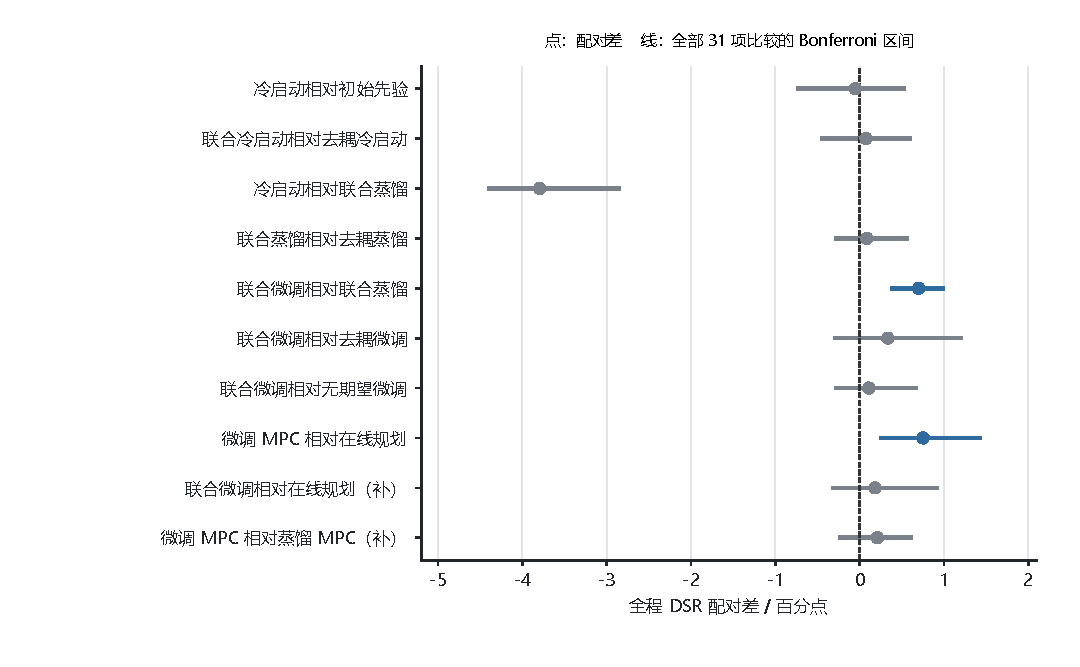
\includegraphics[width=0.99\textwidth]{../docs/figures/ch5_dynamic_04_paired_effects.pdf}
\bicaption{主比较及两项补充比较的全程 DSR 配对差。前八行为原主检验族，末两行用于限定在线替代与 MPC 内部增量。线段统一为31项 DSR 比较的 Bonferroni 区间，蓝色表示区间完全高于零；区间条件于三个固定父谱系}{Paired full-horizon DSR effects with Bonferroni intervals across all 31 comparisons}
\label{fig:ch5-dynamic-effects}
\end{figure}

\subsection{神经引导 MPC 与在线规划参照}

微调 Top-6 MPC 的 DSR 为49.31\%，在线规划基线为48.56\%；前者多完成1898个请求，差0.75个百分点，单比较95\%区间 $[+0.41,+1.16]$，全31项区间 $[+0.25,+1.42]$。结合后文计算成本，这支持在本协议下采用学习引导的有限候选前瞻作为另一种控制选择。

同框架下，先验 Top-6 MPC 为45.46\%，蒸馏 Top-6 MPC 为49.10\%，微调 Top-6 MPC 为49.31\%。学习先验相对初始先验带来较大整体收益，但微调相对蒸馏 MPC 的0.21个百分点差，其95\%区间 $[-0.06,+0.48]$ 跨零。因此不能把结果写成已证实的逐级显著提升，也不能由微调 MPC 相对旧规划基线显著更好，反推微调阶段对 MPC 的独立收益已确立。

零在线前瞻的联合微调相对在线规划基线高0.18个百分点，95\%区间为 $[-0.168,+0.605]$，不支持优效结论。该比较90\%区间为 $[-0.128,+0.523]$，在 $\pm0.50$ 个百分点范围下未通过 TOST 等效判定；95\%区间下界高于 $-0.50$ 个百分点，满足相应非劣效判定。在 $\pm0.75$ 个百分点范围下通过等效判定。这里明确给出容许界值的结果，不把界值视为已有业务标准，也不因选择一个可通过的界值就宣称工程等价已被普遍证明。

\subsection{接纳与接纳后质量的共同变化}

图~\ref{fig:ch5-dynamic-service} 将主要控制方式的生成请求分为按时完成、接纳后失败和未接纳三类，并展示按到达阶段分组的 DSR。联合微调的接纳率为52.58\%，接纳后完成率为92.69\%；在线规划基线约为51.76\%与93.82\%。二者全程 DSR 接近时，联合微调接纳更多请求，而接纳后质量较低。这说明不能用其微小正向 DSR 点估计宣称所有服务质量指标均已改善。

\begin{figure}[!htbp]
\centering
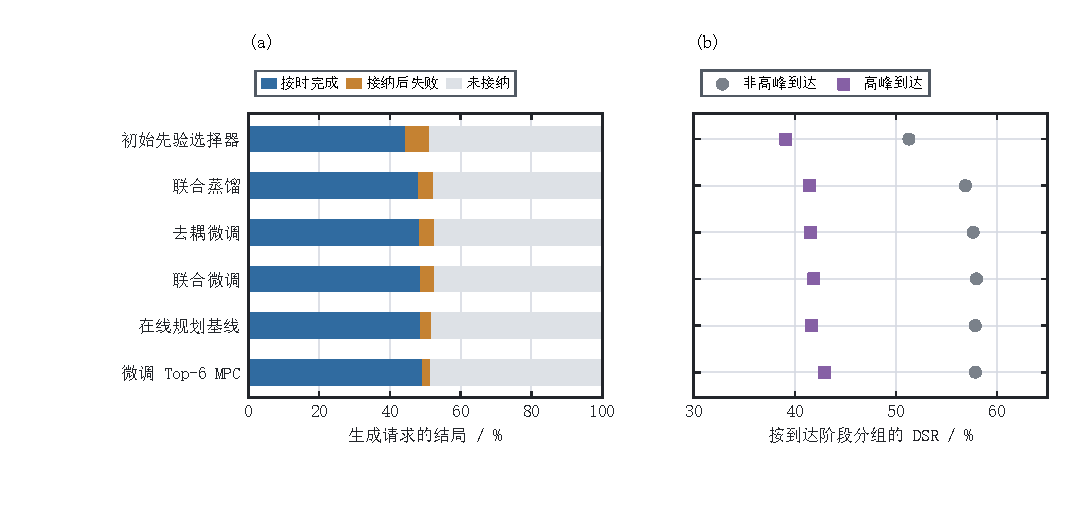
\includegraphics[width=0.99\textwidth]{../docs/figures/ch5_dynamic_05_service_outcomes.pdf}
\bicaption{主要控制方式的请求结局与阶段差异。（a）按生成请求池化的三类结局，未接纳请求同样计入分母；（b）按到达时刻区分高峰与非高峰请求的 DSR，任务结算包含后续排空。六种方法用于说明服务构成，完整十七臂结果见表~\ref{tab:ch5-dynamic-main}；本图为描述性结果，不作新的多重检验声明}{Request outcomes and arrival-cohort DSR for six representative controls}
\label{fig:ch5-dynamic-service}
\end{figure}

联合微调相对去耦微调的全程条件完成率约高0.89个百分点，但两者接纳的并不是完全相同的请求群体。该比率可以提示准入与执行质量的取舍，不能直接解释为对相同任务的因果质量提升。高峰到达组在各控制方式下仍明显困难，说明学习改进未消除突发负载与有限物理资源之间的矛盾。

\subsection{平均计算开销与尾延迟}

表~\ref{tab:ch5-dynamic-cost} 和图~\ref{fig:ch5-dynamic-cost} 同时报告平均耗时与尾部行为。联合微调平均每步0.520秒，在线规划基线1.602秒，均值比约3.08；微调 Top-6 MPC 为0.722秒，比基线约低55\%。在线规划基线累计记录1664565个确定性 Engine 步，联合微调两类在线前瞻计数均为零，微调 Top-6 MPC 记录58173个预测候选分支。

\begin{table}[!htbp]
\centering\small
\bicaption{主要控制方式的平均耗时、尾延迟与前瞻计数}{Decision time, tail latency and lookahead counters}
\label{tab:ch5-dynamic-cost}
\begin{tabular}{lrrrrr}
\toprule
方法 & 均值/s & p95/s & $>1$s/\% & 确定性步数 & 预测分支数 \\
\midrule
初始先验选择器 & 0.463 & 1.275 & 16.6 & 0 & 0 \\
联合蒸馏 & 0.439 & 1.220 & 15.0 & 0 & 0 \\
联合微调 & 0.520 & 1.297 & 16.9 & 0 & 0 \\
先验 Top-6 MPC & 0.692 & 2.166 & 24.3 & 0 & 58147 \\
蒸馏 Top-6 MPC & 0.711 & 2.196 & 24.4 & 0 & 58161 \\
微调 Top-6 MPC & 0.722 & 2.203 & 24.5 & 0 & 58173 \\
在线规划基线 & 1.602 & 5.998 & 29.7 & 1664565 & 0 \\
\bottomrule
\end{tabular}
\par\vspace{0.4em}\begin{minipage}{0.96\textwidth}\footnotesize 计时来自本轮评估记录，不是隔离硬件基准。预测分支使用Engine克隆推进，但记在预测分支计数中，不能把其确定性计数为零理解为没有仿真。物理环境未计入墙钟等待。\end{minipage}
\end{table}


\begin{figure}[!htbp]
\centering
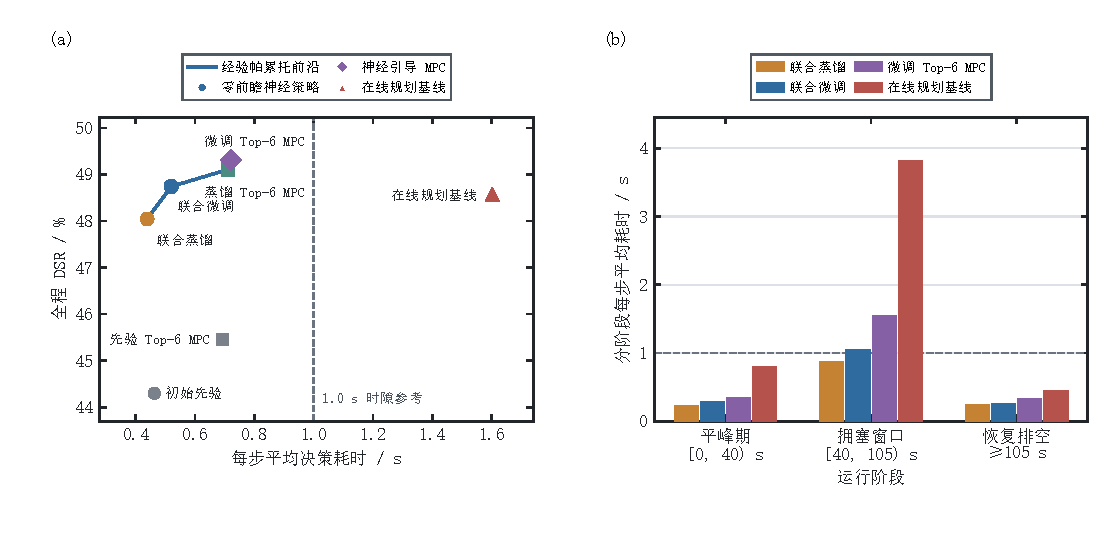
\includegraphics[width=0.99\textwidth]{../docs/figures/ch5_dynamic_06_decision_cost.pdf}
\bicaption{七种主要控制方式的决策耗时。（a）本轮评估记录的均值与p95；（b）超过1秒的决策比例。数据来自完整调用路径，非隔离硬件时延基准。较低均值不能消除超时风险，且仿真未把墙钟等待加入任务期限演化}{Mean, p95 and one-second exceedance of recorded decision time}
\label{fig:ch5-dynamic-cost}
\end{figure}

联合微调与微调 Top-6 MPC 的 p95 分别为1.297秒和2.203秒，超过一秒的比例分别为16.9\%和24.5\%。这些记录支持当前运行条件下的平均计算成本降低，但不支持硬实时部署。并行评估时的资源竞争、实现语言和硬件会影响墙钟耗时，不能将均值比视为硬件无关的算法常数。物理仿真也未等待计算结束才推进请求，因此一旦把真实决策延迟加入系统，DSR 需要另行评估。

\section{讨论与本章小结}
\label{sec:ch5-discussion}

本章结果支持一种把规划知识与环境交互分工使用的控制思路。蒸馏提供能够利用候选库的起点，完整微调方案进一步提高学生的闭环成功率；当允许在线推演时，学习先验与少量候选评价形成另一种性能和计算成本组合。它们的作用建立在当前候选支持、公开信息和动态排队协议上，不依赖把每个网络组件都解释为已经显著有效。

方法的限制也来自这些设计本身。教师及解析特征携带模型误差，反事实三步分支采用预测到达和固定延续策略，辅助评分与真实轨迹回报不一致，有限候选无法表达任意联合动作。现有消融没有确认耦合相对去耦的独立 DSR 收益，也未隔离辅助评分本身的净贡献。后续若研究这些机制，应固定初始化、优化配置与计算预算，用新负载和新的训练重复作针对性比较，而非直接从本章整体收益推断。

统计结论条件于三个固定父谱系和一个预定突发业务设置，尚未覆盖新父模型重训、不同突发形态或跨算力场景的普遍表现。零在线前瞻也依赖理想的状态收集和集中候选构造。信息上报延迟、字段缺失、控制等待和超时回退若进入环境，将改变可行性与服务结果，属于需要独立评价的新协议。

综上，本章完成了动态排队协议下的规划知识蒸馏、环境交互与反事实辅助 PPO 微调，以及零在线 Engine 前瞻和神经引导 Top-6 MPC 两种控制方式的构建与比较。确认结果支持完整微调方案改善蒸馏学生，支持学习引导 MPC 相对指定规划基线提高 DSR 并降低平均决策开销。与第三、四章结合时，这些结论说明从需求可见性、批量分配到持续排队控制的研究递进；它们不构成把不同协议数值拼接后的统一性能证明，也不包含本章未建模的能量收益。
